

% =============================
% Front matter
\documentclass{kecsmstr}
\usepackage{subfiles}

\usepackage{graphicx}
\graphicspath{ {images/} }
\usepackage{amssymb}
\usepackage{amsfonts}
\usepackage{amsmath}
\usepackage{amsthm}
\usepackage{graphicx} 
\usepackage{musixtex}
\usepackage{tikz}
\usepackage{arev}
%\usepackage{fontspec}
\usepackage{lilyglyphs}
\usepackage{verbatim}
\usepackage{arcs}
\usepackage{gensymb}
\usepackage[lofdepth,lotdepth]{subfig}

\usepackage{unicode-math}
\usepackage{algorithm}
\usepackage[noend]{algpseudocode}

\Umathchardef\xnot="3 \symoperators "0338
\AtBeginDocument{\renewcommand\not[1]{#1\xnot}
\renewcommand{\notin}{\in\xnot}}
\newcommand{\defeq}{\mathrel{\mathop:}=}

\title{Nested Monte Carlo Search with Markov Sampling for First Species Counterpoint}
\author{Roberto Noorduijn Londono}

%select one:
%\thesistype{Master of Science of Knowledge Engineering}
\thesistype{Master of Science of Artificial Intelligence}

\thesisdate{July 2016} \thesisnumber{00-00}

%Thesiscommittee: use \\ to separate members
\committee{Prof.~dr.~????\\
           Prof.~dr.~???? \\
           Dr.~ir. ???? \\
           Dr.~?????}
% ================================


\begin{document}

% leave this in place! =============
\makeheaders \pagenumbering{roman} \maketitle \setcounter{page}{2}
\emptypage
% ================

\chapterx{Preface} \emptypage

\chapterx{Summary} \emptypage

\tableofcontents  \emptypage \pagenumbering{arabic}

\chapter{Introduction}



\documentclass[master.tex]{subfiles} % use larger type; default would be 10pt
\newtheorem*{ps}{Problem Statement}
\newtheorem{researchquestion}{Research Question}
\begin{document}
\section{AI and Music}

The automation of Musical Composition is an endeavor that has intrigued composers for many years. As far back as the 18th century, many attempts were made at making so-called \emph{musical games}. The purpose of these games was to use random events, such as the rolling of a die, to completely determine the compositional process. The most popular of these musical games is one attributed to Mozart, published in 1792 \citeaby{alpern1995techniques}. The game consisted of using die to determine the order of various precomposed sections of music. Although the structure of the final piece would be determined through random events, the actual aesthetic was fully determined by the composer by creating musically pleasing sections that would sound good no matter which order they were played in. That said, such musical games, though trivial, demonstrate the first foray into the field of Algorithmic Composition (AC). 

The term Algorithm Composition refers to the use of algorithmic procedures in order to create music such that the creative involvement from part of the human is minimized. As the years past, many examples chronicled the development of various AC techniques. For example, the serialist movement, a departure from the traditional stances on harmony and melody, gave rise to the twelve tone method as developed by Arnold Schoenberg \citebay{perle1972serial}. A method which used various rules in order to create entirely \emph{atonal} pieces of music.

Unsurprisingly, as computers have advanced, they have allowed for an incredibly wide range of new capabilities within the field of AC. Initially, these methods were predominantly focused around hard coding rules and functions that would determine the structure and content of various pieces. Although these methods become more and more sophisticated, the creative process underlying the piece was still attributed to the formalization of the rules and parameters used. The programmer who determined the rules was still essentially the composer of the piece. With the development of various techniques from Artificial Intelligence (AI), the difference between programmer and composer has become more distinct. This distinction arises from the fact that the programmer does not hard code the rules and creative process but instead allows the program to make the stylistic choices on its own. These advancements have allowed the field of AC to become imbedded within that of Computational Creativity (CC), i.e, the use of computation techniques and algorithms for the purpose of emulating creativity. A wide variety of ideas and techniques have already shared many successes within the domain of musical composition.

\section{Combinatorial Optimization and Counterpoint}
A completed composition can abstractly be seen as the solution to a \emph{combinatorial optimization} problem \citebay{herremans2012composing}. In this regard, the act of composing a piece can be seen as similar to that of writing down a series of \emph{musical events} such that the resulting music maximizes some \emph{objective function}.  Of course, true composition is not so simple. With music, it is difficult to define such an objective function so that the aesthetic quality of a piece can effectively be quantified. While some general rules and heuristics do exist for various styles of music, they tend to not be strict rules and as such are generally suggestions based on experience. 

Species counterpoint is an example of a musical style with strict and rigorous rules. These formal rules allows the possibility of determining an objective function. Generally speaking, counterpoint refers to the use of independent vocal melodies, which are combined to form a harmonious whole. Although when discussing the \emph{style of counterpoint} one is instead referring to the set of principles that were amassed and developed during the Renaissance, in relation to the art of voice polyphony. These principles were then formalized into sets of rules, such that the style of counterpoint could easily be taught by following said rules. The most complete collection of these rules was published by J.J. Fux in 1725 in his \emph{Gradus ad Parnassum}. In here, he describes different \emph{species} of counterpoint and corresponding concise rules to help aid the composition thereof.  

Due to their rigorous formulation, these rules have been implemented and used by many different optimization algorithms in order to determine good solutions to Fuxian counterpoint. An early example is Schottstaedt's approach which made use of search and heuristics derived from these rules \citebay{shottstaedt1989automatic}. However, due to the almost infinite amount of possible melodies one could create - without imposing any restrictions, the majority of recent approaches have focused on stochastic methods. One such example is evolutionary algorithms as shown in \citeay{acevedo2004fugue} and Jacobs (2012). Such methods have proven to be quite successful in generating novel fugues given a starting melody or \emph{cantus firmus}. These approaches are examples of the \emph{generate and test} methods \citebay{togelius2011search}. Pieces are generated, and then tested by using either human evaluation or direct evaluation derived from similar rules as the ones explained above.
Another approach which seems to have a stronger theoretical foundation, is that of reinforcement learning using SARSA (State-Action-Reward-State-Action) \citebay{phon2009generating}. The idea behind this is to model the act of composing music as a Markov Decision Process. States are represented as pitches and the actions are represented as intervals. The rewards of the models are then derived from evaluation criteria which rewards consonant sounds and pitch intervals and penalizes dissonance.  These techniques have all had reasonable success, although they still far short of being considered similar to a human composed piece of music. 
The method proposed by \citeay{chen2001creating} combines both evolutionary algorithms and recurrent neural networks in order to generate new melodies. Melodies were then evaluated using tonal and rhythmic rules, such as tonal and rhythmic diversity. 
In \citebay{collins2011chopin} new music is generated by using Markov Chains analysed from existing compositions. For example, pitch frequencies and their transitions would be recorded and incorporated into a Markov Chain. New pieces would then be made by sampling from this Markov Chain. 

\section{Problem Statement and Research Questions}
Search based methods such as Monte Carlo Search (MCS) have not generally been applied to the task of music generation. The greater focus of methods have relied on stochastic methods such as Markov Chains and Evolutionary Algorithms. Since the task of composing is generally not a random process, but rather can be seen as a more informed (heuristic) search, it appears as though search based methods should be feasible for this problem. Such approaches have been applied with best-first search methods \citebay{shottstaedt1989automatic}, although due to the intractability of the problem, they have not been as successful as the stochastic methods. Based on their previous successes in similar domains, MCS based methods are therefore expected to produce pieces of equal if not greater quality then those of the more popular stochastic methods. The problem statement of this thesis is thus: 

\begin{ps}
Are Monte Carlo Search based approaches viable to the domain of Automated Musical Composition?
\end{ps}
Thus the purpose of the thesis will be to investigate how well MCS based techniques fare compared to the state of the art techniques currently used. In particular, these techniques will be applied in order to create music in the style of First Species Counterpoint. This problem statement will be addressed by answering the following research questions. 

\begin{researchquestion}
How do Monte Carlo based approaches compare to Genetic Algorithms within this domain? 
\end{researchquestion}



\begin{researchquestion}
What is a suitable representation for music within the context of counterpoint?
\end{researchquestion} 

In searching the space of counterpoint efficiently, it is necessary to have a concise representation in order to represent music as points within a specific state-space. Such a representation will effectively require a formalization of important musical concepts. In representing music, there exists a spectrum between direct  or explicit representations and more indirect or implicit representations. An example of a direct representation would be a collection of MIDI information. That is, the pitch, duration, velocity (loudness) and attack time of a particular music event (e.g. a note played on a piano). A slightly more implicit approach would be to only model aspects such as relative pitches between notes, consonance and chord progression. An example of a representation in the more extreme implicit end of the spectrum would be that described by the \emph{Generative Theory of Tonal Music}, a grammatical hierarchical approach to music representation. This representation deals more with the cognitive aspects of music theory and thus is generally more difficult to implement. \citebay{tojo2013computational} describe a method for automatically analyzing music according to this theory. It is expected that an approach that lies somewhere in between would be the most appropriate as it is necessary to have a more direct representation in order to simplify the task of searching, but also it would be necessary to encode more information in order to represent more complex relationships inherent in the music. 

\begin{researchquestion}
How can the contrapuntal pieces be evaluated?
\end{researchquestion}

As discussed earlier, the evaluation of music is difficult problem. The main approach in this thesis will be to take the qualitative rules of first species counterpoint and turn them in quantitative measures.  Other approaches to determining a feasible evaluation will also be researched. These include using features learned from a corpus of pre-existing music and seeing how closely the generated music resembles music from the corpus. 

Since the actual fitness of a peice of music tends to be a subjective matter, the results will have to be evaluated using human participants. To this extent the various results from the different techniques and evaluation functions will be used in a survey carried out on a number of people with varying musical maturity. The purpose of such a survey will thus be to truly see how well the different pieces sound. The results of this survey will also be able to answer another research question: 

\begin{researchquestion}
Using just the rules derived from first species counterpoint, how good are the pieces generated?
\end{researchquestion}

Due to species counterpoint being mainly a pedagogical tool that was created in order to aid students in the understanding of contrapuntal composition, it has never been a standard under which music is actually composed. The main reason for this is the fact it is very difficult to ensure that all the rules have been satisfied. It is also especially difficult for even an expert, to be able to listen to a piece of species counterpoint and determine whether it satisfies all the rules. Given that an appropriate formalization of the rules have been determined, it is expected that a piece of music that obtains the highest fitness value from the evaluation function should represent the best piece of species counterpoint. Therefore, under the previous assumption, the survey test will serve to reveal whether or not these rules do in fact create aesthetically pleasing music. 

\begin{researchquestion}
Can Markov Chains be used in order to improve the MCS methods?
\end{researchquestion}

The purpose of this thesis is to investigate different techniques from AI applied to the problem of \emph{first species counterpoint}. In particular, a new method based on Nested Monte Carlo Search (NCMS) will be proposed and compared to existing techniques from the literature. This problem will be addressed by describing the exact rules that will be used for evaluation, discussing the representation and then setting up the proposed algorithm 

\section{Outline}








\end{document}


\chapter{Music Theory}

\documentclass[master.tex]{subfiles}


\newcommand{\setmeterb}[2]{\ensuremath{%
  \vcenter{\offinterlineskip
    \halign{\hfil##\hfil\cr
            $\scriptstyle#1$\cr
            \noalign{\vskip1pt}
            $\scriptstyle#2$\cr}
  }}%chen2001creating
}
\begin{document}




Music theory is the based on the analysis of music. This typically reflects an analysis of different fundamental aspects of music. These include melody, harmony, rhythm and form. The following sections aim to introduce these concepts. Though music theory has developed to encompass many different forms of music, for the purpose of this research, the concepts introduced will be those that are in relation to the traditions of Western music. 
\section{Pitch}
Pitch is a perceived property of sound directly related to frequency. It is the quality of sounds that allows us to distinguish between higher and lower sounds. When a string vibrates at a frequency of 440hz this is referred to as the pitch \rmfamilyA. Though pitch is related to frequency, human perception of pitch depends not linearly on frequency but rather logarithmically. Therefore, the difference between 220hz and 440hz sounds is perceived as the same difference between 130.81hz and 261.63hz. Such a difference between pitches is called an \emph{interval}. In particular, the intervals just described are denoted as an \emph{octave}. Octaves are special intervals as they can be used to partition pitches into equivalence classes. The following demonstrates how to do this. Let $\sim$ be a binary relation such that:
\begin{equation}
    a \sim b \equiv \frac{a}{b} = 2^{k} \quad \textnormal{for some} \quad k \in \mathbb{Z}
\end{equation}
Clearly, $\sim$ is an equivalence relation for the space of frequencies. Equivalence classes thus represent similar sounding tones and are therefore denoted by the same letter. When one refers to {A}, one is actually referring to a collection of different pitches ${[}\textnormal{{A}}{]} = \{\dots, 55, 110, 220, 440, 880, 1760 \ldots\}$. These equivalence classes are typically called \emph{pitch classes}. Although the space of possible frequencies is a continuum of different values, typical {Western} music theory only deals with a finite subset of frequencies represented by 12 different pitch classes. The pitch classes are referred to as {A, A\#, B, C, C\#, D, D\#, E, F, F\#, G, G\#}. Since pitches are on a logarithmic scale, they can be transformed into a linear scale with the following function:
\begin{equation}
    M(x) = 69 + 12\log_2\frac{x}{440}
\end{equation}
$M(440) = 69$ and $M(220) = 57$ (seeTable \ref{freqtable}). In this scale, the difference between two adjacent pitches is called a \emph{semitone}. In order to distinguish between different tones of the same pitch class, i.e, {A} at 440hz and {A} at 220hz, we use the \emph{Scientific Pitch Notation}. In this notation we use a number suffix to represent whether a tone is higher or lower, see the table \ref{freqtable}.

The value of a pitch can be altered  by using \emph{accidentals}. These are shown by the symbols $\flat$ and $\sharp$. Writing $\flat$ next to a pitch lowers the pitch by a semi-tone, whereas $\sharp$ raises it by a semitone. 
\begin{table}[]
\centering
\caption{Relations between Pitch, Pitch class and Frequency}
\label{freqtable}
\renewcommand{\arraystretch}{2}
\begin{tabular}{c|c|c|c|c|c}

\hline
\multicolumn{1}{l|}{\textbf{Pitch}} & \multicolumn{1}{l|}{\textbf{Pitch Class}} & \multicolumn{1}{l|}{\textbf{Freq (hz)}} & \multicolumn{1}{l|}{\textbf{$M(x)$}} & \multicolumn{1}{l|}{\small\textbf{Freq. diff.}} & \multicolumn{1}{l}{\small\textbf{$\log_2 (\textnormal{\textbf{Freq. diff.}})$}} \\ \hline
\textbf{A3}                         & \textbf{A}                                & 220                                     & 57                                   & -                                              & -                                                                   \\
\textbf{A\#3}                       & \textbf{A\#}                              & 233.08                                  & 58                                   & 13.08                                          & $\frac{1}{12}$                                                      \\
\textbf{B3}                         & \textbf{B}                                & 246.94                                  & 59                                   & 13.86                                          & $\frac{1}{12}$                                                      \\
\textbf{C4}                         & \textbf{C}                                & 261.63                                  & 60                                   & 14.69                                          & $\frac{1}{12}$                                                      \\
\textbf{C\#4}                       & \textbf{C\#}                              & 277.18                                  & 61                                   & 15.55                                          & $\frac{1}{12}$                                                      \\
\textbf{D4}                         & \textbf{D}                                & 293.66                                  & 62                                   & 16.48                                          & $\frac{1}{12}$                                                      \\
\textbf{D\#4}                       & \textbf{D\#}                              & 311.13                                  & 63                                   & 17.47                                          & $\frac{1}{12}$                                                      \\
\textbf{E4}                         & \textbf{E}                                & 329.63                                  & 64                                   & 18.50                                          & $\frac{1}{12}$                                                      \\
\textbf{F4}                         & \textbf{F}                                & 349.23                                  & 65                                   & 19.60                                          & $\frac{1}{12}$                                                      \\
\textbf{F\#4}                       & \textbf{F\#}                              & 369.99                                  & 66                                   & 20.76                                          & $\frac{1}{12}$                                                      \\
\textbf{G4}                         & \textbf{G\#}                              & 392.00                                  & 67                                   & 22.01                                          & $\frac{1}{12}$                                                      \\
\textbf{G\#4}                       & \textbf{G\#}                              & 415.00                                  & 68                                   & 23.00                                          & $\frac{1}{12}$                                                      \\
\textbf{A4}                         & \textbf{A}                                & 440.00                                  & 69                                   & 24.00                                          & $\frac{1}{12}$                                                      \\ \hline
\end{tabular}
\end{table}

%Staff notation provides a way of representing music visually. Each line and space represents a different pitch. The image \ref{notation} shows some pitches and their locations on the staff.    
%Insert picture for notation here

\section{Scales}
Let the set of all pitch classes be given by $\Omega = $ \{{A, A\#, B, C, C\#, D, D\#, E, F, F\#, G, G\#}\}. A \emph{scale} is any non-empty ordered subset $S \subseteq \Omega$. The scale $S = \Omega$ is called the \emph{chromatic} scale. Scales are typically used to represent the types of pitches used in a piece of music. Although a musical piece may use one scale, one can use other pitches through the use of accidentals mentioned above. 

Of great importance to early Western music are the \emph{Diatonic} scales. These are scales which consists of 7 different pitches and can be split into the \emph{major} and \emph{minor} scales. For each of the pitch classes, there is a distinct diatonic scale defined which uses that pitch class as its starting point, also called the \emph{tonic}. 

\begin{table}[]
\centering
\caption{Scale Degrees for the C major key}
\label{scaledegrees}
\renewcommand{\arraystretch}{1.5}
\begin{tabular}{|c|c|l|}
\hline
\textbf{Pitch} & \multicolumn{2}{c|}{\textbf{Scale Degree}} \\ \hline
C              & Tonic                  & $\hat{1}$           \\
D              & Supertonic             & $\hat{2}$           \\
E              & Mediant                & $\hat{3}$           \\
F              & Sub-dominant           & $\hat{4}$           \\
G              & Dominant               & $\hat{5}$           \\
A              & Sub-mediant            & $\hat{6}$           \\
B              & Leading note           & $\hat{7}$           \\ \hline
\end{tabular}
\end{table}

An invariant feature among all different diatonic scales are the amount of semi-tones - or intervals - between consecutive pitches. For example, the diatonic {C} major scale is given by the pitches \{{C, D, E, F, G, A, B}\} while the {G} major scale is given by \{{G, A, B, C, D, E, F\#}\}. Examining these scales, one can see that the number of semi-tones between consecutive pitches are \{2, 2, 1, 2, 2, 2, 1\} where the final semi-tone is the transition from the final pitch to the starting note, one octave up. The interval differences for the diatonic minor scales are given by \{2, 1, 2, 2, 1, 2, 2, 2\}. Using these differences one can see that the {A} minor scale is given by \{{A, B, C, D, E, F, G}\}. Since {C} major and {A} minor share the same pitches, {A} minor is called the \emph{relative minor} of {C} major. Similarly, {C} major is the \emph{relative major} of {A} minor. 

Within these diatonic scales, each pitch is given a particular name referred to as the \emph{scale degree}. These scale degrees reflect the different qualities and functions of the pitches within a certain scale. Table \ref{scaledegrees} shows the scale degrees corresponding to the pitches in the C major scale. The tonic, sub-dominant and dominant are particularly important scale degrees and their functions will be discussed in more detail later. 

\section{Intervals}
As discussed above, intervals measure the distance between two pitches. While intervals can be measured using the semi-tone distance between pitches, it is clearer to refer to refer to intervals relative to their positions in a specific scale. The following shows the intervals relative to C in the C major scale. 
\begin{itemize}
    \item C $\rightarrow$ D, 2 semitones, \textbf{major second}
    \item C $\rightarrow$ E, 4 semitones, \textbf{major third}
    \item C $\rightarrow$ F, 5 semitones, \textbf{perfect fourth}
    \item C $\rightarrow$ G, 7 semitones, \textbf{perfect fifth}
    \item C $\rightarrow$ A, 9 semitones, \textbf{major sixth}
    \item C $\rightarrow$ B, 11 semitones, \textbf{major seventh}
    \item C $\rightarrow$ C, 12 semitones, \textbf{octave}
\end{itemize}
Other intervals are possible. Minor intervals are those which are a semi-tone less then major intervals, such as the minor third C $\rightarrow$ E$\flat$. Augmented intervals raise the value of perfect intervals by one semitone while diminished intervals lower the value by one semitone.

\section{Chords}
A chord is a combination of 3 or more pitches sounding simultaneously. The most basic type of chord is the \emph{triad}, composed of 3 pitches. Each triad is built off a base pitch or \emph{root} and two intervals above the root. There are 4 different types of triads. 
\begin{itemize}
    \item \textbf{Major Triad} - root, major third and perfect fifth, e.g., a C maj. = (C, E, G). 
    \item \textbf{Minor Triad} - root, minor third and perfect fifth, e.g., a C min. = (C, E$\flat$, G)
    \item \textbf{Augmented Triad} - root, major third and augmented fifth, e.g., a C aug. = (C, E, G$\sharp$)
    \item \textbf{Diminished Triad} - root, minor third and diminished fifth, e.g., a C dim = (C, E$\flat$, G$\flat$)
\end{itemize} 
Another type of chord are the seventh chords. These are essentially the same as the triads, except with added augmented or diminished seventh interval. 
Chords do not strictly need to be played with the closest pitches, for example the C major key need not consist of the pitches (C4, E4 G4), but they can be (E2, G3, C4). The process of separating pitches over wider registers is called \emph{voicing}. Voicing corresponds to the act of assigning separate voices or instruments to different parts of a chord. 

\section{Duration}
Another important property of perceived sound, is that of duration. As the name implies, duration refers to the amount of time for which a particular sound persists. A pitch with a specified duration is referred to as a \emph{note}. In music, duration is measured in terms relative to the whole note \hspace{0.1cm} \wholeNote \hspace{0.2cm}which has a duration of 1 (see Table \ref{durations}). Lack of notes are represented in music using rests.

\begin{table}[]
\centering
\caption{Durations of Notes and Rests}
\label{durations}
\renewcommand{\arraystretch}{1.5}
\begin{tabular}{c|c|c|c}
\hline
\textbf{Symbol}   & \textbf{Name}     & \textbf{Duration} & \textbf{Equivalent Rest} \\ \hline
\wholeNote        & whole note        & 1                 & \wholeNoteRest           \\
\halfNote         & half note         & $\frac{1}{2}$     & \halfNoteRest            \\
\quarterNote      & quarter note      & $\frac{1}{4}$     & \quaverRest              \\
\eighthNote       & eighth note       & $\frac{1}{8}$     & \semiquaverRest          \\
\sixteenthNote    & sixteenth note    & $\frac{1}{16}$    & \lilyGlyph{rests.5}    \\
\thirtysecondNote & thirtysecond note & $\frac{1}{32}$    & \lilyGlyph{rests.6}    \\ \hline
\end{tabular}
\end{table}

The length of notes can be extended through two principle ways. The first way is by use of the $\cdot$ operator. When placed next to a note, the dot operator increases the duration of that note by half its original duration. Thus \halfNoteDotted has a duration equal to $\frac{3}{4}$. Similarly the duration of \semiquaverDotted has a duration of $\frac{3}{32}$. The other way of increasing the duration of a note is by \emph{tying} them together. Tying notes has the effect of adding the duration all of tied notes together. For example the duration of \underarc{\halfNote \hspace{0.5cm}\eighthNote} is $\frac{1}{2} + \frac{1}{8} = \frac{5}{8}$. 
Patterns of varying durations and rests give rise to the phenomenon known as \emph{rhythm}. 

\section{Music Notation} 
Music is typically represented using \emph{Staff Notation}. It provides an organizational method that allows music to be read from left to right. A Staff consists of 5 lines and 4 spaces. Each line and space corresponds to a different pitch. Clefs are used to assign specific values to each position. The treble clef \clefGInline \hspace{0.1cm}  assigns the value of G4 to the second line from the bottom, while the bass clef \clefFInline \hspace{0.1cm} assigns the value of F3 to fourth line from the top. Ledger lines are used to represent pitches that do not fit on the staff lines. See the following figures below (\ref{fig:subfig1}, \ref{fig:subfig2}). 

\begin{figure}[h]
\subfloat[Treble Clef Notes][Treble Clef]{

\label{fig:subfig1}
\begin{music}\nostartrule
\parindent10mm
\instrumentnumber{1}
\setstaffs1{1}
\startextract
\Notes \zcharnote{-10}{A3}\wh a \en
\Notes \zcharnote{-9}{B3}\wh b \en
\Notes \zcharnote{-8}{C4} \wh c \en
\Notes \zcharnote{-7}{D4} \wh d \en
\Notes \zcharnote{-6}{E4} \wh e \en
\Notes \zcharnote{-5}{F4} \wh f \en
\Notes \zcharnote{-4}{\textbf{G4}} \wh g \en
\Notes \zcharnote{-3}{A4} \wh h \en
\Notes \zcharnote{+8}{B4} \wh i\en
\Notes \zcharnote{+9}{C5} \wh j \en
\Notes \zcharnote{+10}{D5} \wh k \en
\Notes \zcharnote{+11}{E5} \wh l \en
\Notes \zcharnote{+12}{F5} \wh m \en
\Notes \zcharnote{+13}{G5} \wh n \en
\Notes \zcharnote{+14}{A5} \wh o \en
\zendextract
\end{music}
}

%\begin{subfigure}
%\caption{Bass Clef}
\subfloat[Bass Clef Notes][Bass Clef]{
\begin{music}\nostartrule
\parindent10mm
\instrumentnumber{1}
\setstaffs1{1}
\setclef1\bass
\startextract
\Notes \zcharnote{-10}{E2}\wh E \en
\Notes \zcharnote{-9}{F2}\wh F \en
\Notes \zcharnote{-8}{G2} \wh G \en
\Notes \zcharnote{-7}{A2} \wh H \en
\Notes \zcharnote{-6}{B2} \wh I \en
\Notes \zcharnote{-5}{C3} \wh J \en
\Notes \zcharnote{-4}{D3} \wh K \en
\Notes \zcharnote{-3}{E3} \wh L \en
\Notes \zcharnote{+8}{\textbf{F3}} \wh M\en
\Notes \zcharnote{+9}{G3} \wh N \en
\Notes \zcharnote{+10}{A3} \wh O \en
\Notes \zcharnote{+11}{B3} \wh P \en
\Notes \zcharnote{+12}{C4} \wh Q \en
\Notes \zcharnote{+13}{D4} \wh R \en
\Notes \zcharnote{+14}{E4} \wh S \en
\zendextract
\end{music}
\label{fig:subfig2}
}
\caption{Staff notes with treble and bass clef}.
\label{fig:globfig}
\end{figure}

Chords are represented by writing the notes of which it consists of on top of one another. Accidentals (\flat, \sharp) are used to denote other pitches then the ones shown in figures \ref{fig:subfig2} and \ref{fig:subfig1}. For an example of accidentals, see figure \ref{fig:chords}.
 
\begin{figure}[h!]
\caption{Examples of chords and accidentals in staff notation}

\begin{music}\nostartrule
\parindent10mm
\instrumentnumber{1}
\setstaffs1{1}
\startextract
\NOTEs \zcharnote{-7}{C min.}\zw{c_eg}\en
\NOTEs \zcharnote{-7}{D maj.}\zw{d^fh} \en
\NOTEs \zcharnote{-7}{F aug.}\zw{fh^j}  \en
\NOTEs \zcharnote{-7}{E dim.}\zw{eg_i } \en
\zendextract
\end{music}
\label{fig:chords}
\end{figure}


Vertical lines divide up the Staff into bars or measures. The length of these measures is determined by the two numbers next to the clefs. These two numbers represent a fraction that determine the length of the bar in terms of whole notes. These two numbers are called the \emph{meter} of a piece. Thus, if the meter is \lilyTimeSignature{4}{4}, then each bar lasts for the same duration as a whole note. It should be noted that, although there is a difference between similar meters such as \lilyTimeSignature{4}{4} and \lilyTimeSignature{2}{2}, such a discussion is beyond the scope of this chapter. Figure \ref{fig:mozart} shows an extract from a piece of music in \lilyTimeSignature{4}{4}. \\

\begin{figure}[h!]
\caption{First two bars of W.A. Mozart's \emph{Piano Sonata No. 16 in C Major}}
\label{fig:mozart}
\begin{music}
\parindent10mm
\instrumentnumber{1} % a single instrument
\setname1{Piano} % whose name is Piano
\setstaffs1{2} % with two staffs
\generalmeter{\meterfrac44}% 4/4 meter chosen
\nobarnumbers
\startextract % starting real score
\Notes \zcharnote{-7}{(2)} \ibu0f0\qb0{cge}\tbu0\qb0g| \zcharnote{-5}{(1)}\hl j\en
\Notes\ibu0f0\qb0{cge}\tbu0\qb0g|\ql l\sk\ql n\en
\xbar
\Notes\ibu0f0\qb0{dgf}|\qlp i\en
\notes \tbu0\qb0g|\zcharnote{+10}{(3)}\ibbl1j3\qb1j\tbl1\qb1k\en
\Notes\ibu0f0\qb0{cge}\tbu0\qb0g|\hl j\en
\zendextract % terminate excerpt
\end{music}
\end{figure}


Inspecting figure \ref{fig:mozart} one can see that the two staffs are linked by use of vertical bar lines. This implies that the music contained in both bars is to be played simultaneously. The note at position (1) is the same as the standard \halfNote \hspace{0.2cm} although it is written upside down for aesthetic reasons. At (2) eighth notes \eighthNote \hspace{0.1cm} are linked together by use of a \emph{beam}. This is done to aid legibility of notes and to link together groups of notes that form a natural \emph{phrase}. 

\section{Melody}

A phrase or melody is a collection of successive notes that are that are perceived as a whole within a piece of music. Melodies are typically described by the intervals between successive notes as well as by its rhythm. A way of characterizing the overall structure of a melody is through its \emph{contour}. The contour of a melody refers to the movement of the melody as well as the proximity between consecutive notes. An \emph{ascending} melody is one in which pitches between consecutive notes is increasing, \emph{descending} when the pitches decrease and \emph{undulating} refers to when there is equal movement upwards and downwards. The proximity of a phrase can be described as either \emph{conjunct} or \emph{disjunct}. If a phrase is conjunct that means that intervals between notes are only seconds (major or minor, see the section on intervals) also called \emph{steps}. Conversely, disjunct means that that the interval between two consecutive notes is anything but a second, also called \emph{skips}.  

In Western music, melodies are usually played within one specific scale. When analysing a melody, one also pays attention to the role of the various pitches within a particular scale according to their diatonic function. For example, the tonic of a scale is considered the tonal home and thus usually provides a good starting and ending point for a melody. The dominant of a scale usually represents an increase in tension which can be resolved by tending back towards the tonic. Typically, notes with a particular function are played on a beat to emphasize their role. Notes whose purpose are only transitional between these functional notes are called \emph{passing notes}. 

\section{Harmony}
Harmony refers to the quality of music that is percieved when multiple pitches or voices are sounding. Harmonic analysis is generally built on the analysis of chords through \emph{chord progressions} and \emph{cadences}. 

A chord progression is a sequence of chords within a particular piece. These sequences are typically understood in terms of diatonic chords and triads. Diatonic triads are special triads that are built within a given diatonic scale (major or minor). For each scale degree, a different triad is built on it, using that pitch as it's root, the third pitch above the root in the scale as the middle pitch and the fifth pitch above the root as the top pitch. These triad are identified using roman numerals, corresponding to the scale degree of the root note. A capital roman numeral indicates that the triad is major, while a lower case one indicates that it is minor. A plus sign is used to indicate that the triad is an augmented one while a circle ($\degree$) indicates that it is diminished. 

\begin{figure}[h]
\subfloat[C Major Scale and Diatonic Chords][C major Scale]{
\label{fig:subfig3}
\begin{music}
\parindent10mm
\nobarnumbers
\instrumentnumber{1}
\setstaffs1{1}
\startextract
\NOtes \zcharnote{-7}{$\hat{1}$}\wh c \en
\NOtes \zcharnote{-7}{$\hat{2}$}\wh d \en
\NOtes \zcharnote{-7}{$\hat{3}$}\wh e \en
\NOtes \zcharnote{-7}{$\hat{4}$}\wh f \en
\NOtes \zcharnote{-7}{$\hat{5}$}\wh g \en
\NOtes \zcharnote{-7}{$\hat{6}$}\wh h \en
\NOtes \zcharnote{-7}{$\hat{7}$}\wh i \en \xbar
\NOtes \zcharnote{-7}{I}\zw {ceg} \en
\NOtes \zcharnote{-7}{ii}\zw {dfh} \en
\NOtes \zcharnote{-7}{iii}\zw {egi} \en
\NOtes \zcharnote{-7}{IV}\zw {fhj} \en
\NOtes \zcharnote{-7}{V}\zw {gik} \en
\NOtes \zcharnote{-7}{vii}\zw {hjl} \en
\NOtes \zcharnote{-7}{viii\degree}\zw {ikm} \en
\zendextract
\end{music}
}

\subfloat[C Minor Scale and Diatonic Chords][C Minor Scale]{
\label{fig:subfig4}
\begin{music}
\parindent10mm
\instrumentnumber{1}
\setstaffs1{1}
\nobarnumbers
\startextract
\NOtes \zcharnote{-7}{$\hat{1}$}\wh c \en
\NOtes \zcharnote{-7}{$\hat{2}$}\wh d \en
\NOtes \zcharnote{-7}{$\hat{3}$}\wh {_e} \en
\NOtes \zcharnote{-7}{$\hat{4}$}\wh f \en
\NOtes \zcharnote{-7}{$\hat{5}$}\wh g \en
\NOtes \zcharnote{-7}{$\hat{6}$}\wh {_h} \en
\NOtes \zcharnote{-7}{$\hat{7}$}\wh {_i} \en \bar
\NOtes \zcharnote{-7}{i}\zw {c_eg} \en
\NOtes \zcharnote{-7}{ii\degree}\zw {df_h} \en
\NOtes \zcharnote{-7}{III}\zw {_eg_i} \en
\NOtes \zcharnote{-7}{iv}\zw {f_hj} \en
\NOtes \zcharnote{-7}{v}\zw {g_ik} \en
\NOtes \zcharnote{-7}{VII}\zw {_hj_l} \en
\NOtes \zcharnote{-7}{VIII}\zw {_ikm} \en
\zendextract
\end{music}
}
\caption{Diatonic Chords with Roman Numbering} 
\end{figure}

A chord progression is thus identified by a sequence of identifiers, eg, I $\rightarrow$ IV $\rightarrow$ V $\rightarrow$ I.  Of particular interest are chord progressions known as \emph{cadences}.
These are chord progressions that sound to create a sense of \emph{resolution} and, as such, are usually used to signify the end of a phrase or a piece of music. There are four main types of cadences:
\begin{itemize}
\item \textbf{Authenic Cadence} (V $\rightarrow$ I): This cadence has a strong sense of resolution as it alternates between the dominant (tension) and the tonic (home). 
\item \textbf{Half Cadence}: A half cadence refers to any cadence that ends of on V. Since it ends on the dominant, it has the weakest sense of resolution of all cadences and thus has a strong desire for continuation (towards a resolution). It is called a half cadence as its ending chord is half of the authentic cadence. 
\item \textbf{Plagal Cadence} (IV $\rightarrow$ I): A cadence which involves the subdominant and the tonic. Since the subdominant is tonally less tense than the dominant, such a cadence has a weaker resolution than the authentic cadence. 
\item \textbf{Deceptive or Interrupted Cadence} (V $\rightarrow$ vi): The deceptive cadence is one which gives the listener a suspended feeling as it is very close to the authentic cadence but does not ultimately resolve to the tonic. 
\end{itemize}

Another important aspect of harmony is that of \emph{consonance} and \emph{dissonance}. The difference between consonance and dissonance can vaguely be described as that which sounds ''good'' versus that which doesn't and, as such, is highly context dependant. Something that may sound dissonant in one culture could be consonant in another. One usually refers to consonance in relation to notes being played together (although one could talk about consonant rhythms and melodies). In western music, all perfect intervals (the octave, fifth and fourth) as well as the thirds and sixths (major and minor), all other intervals are considered dissonant. Though dissonance implies that something may not sound  ''good'', it plays a pivotal role in tension building within music with dissonances typically being resolved to consonances. 

% add example of consonance 
\section{Counterpoint}
Counterpoint refers to the relation between different voices that are independent melodically yet come together harmonically to form a whole. The process of writing counterpoint is generally considered a difficult one as, for each melody, each note serves a dual purposes; melodically and harmonically. Species counterpoint is a form of \emph{strict} counterpoint, in which counterpoint on a given melody, or \emph{cantus firmus}, is created by following a series of rules.

% add example of counterpoint 
\begin{figure}[h!]
\caption{Counterpoint}
\begin{music}
\parindent10mm
\instrumentnumber{1}
\setstaffs1{2}
\startextract
\NOtes \wh c |\wh j\en  
\NOtes \wh{_e} |\wh g\en 
\NOtes \wh f |\wh{_h}\en 
\NOtes \wh d|\wh{i} \en 
\NOtes \wh c|\wh{j} \en \Endpiece
\zendextract
\end{music}
\label{fig:counterpoint}
\end{figure}

When discussing counterpoint, one usually refers to the resulting motion between two different voices. This motion can be characterized in 4 ways.
\begin{itemize}
\item \textbf{Parallel motion}: The voices move in a similar direction, mainting the same interval between notes.
\item \textbf{Similar motion}: The voices is move in a similar direction, although the interval between notes changes. 
\item \textbf{Contrary motion}: The voices move in exactly opposite directions. When one voice moves up, the other one moves down.
\item \textbf{Oblique motion}: One voice moves while the other remains on the same note. 
\end{itemize} 

The following describe some of the most important rules used within species counterpoint: 

\begin{itemize}
\item Avoid unisons (except at beginning or end of the piece)
\item Prioritise contrary motion
\item Begin and end on perfect consonance (except for a fourth)
\item Do not move in parallel fourths
\item Do not move too much in parallel thirds and sixths
\item Approach perfect consonances by oblique or contrary motion
\item Intervals should not exceed more than a tenth
\end{itemize}

More rules are described for different \emph{species} of counterpoint. The above rules are applied for when the two melodies fall exactly one on top of the other. Other rules need to be taken into account when the rhythmic structure of the two voices differ. 

\section{Imitation}
In music, imitation refers to the repitition of a melody in a different voice in close successsion. Typically a voice will start with the melody, shortly followed by another voice playing the same melody and so on.
The melody may be repeated as is, resulting in \emph{real} imitation, or it may be altered according to one or more transformations. These are as follows:
\begin{itemize}
\item \textbf{Inversion}: The intervals between notes are inverted. The inversion $i'$ of an interval $i$ can be calculates as follows: $i' = 12 - i$. Therefore if an interval consists of a perfect fifth $i$ = 7, then the inverted interval is $i' = 5$, a perfect fourth. 
\item \textbf{Retrograde}: The melody is played backwards. The rhythmic structure of the original melody can be maintained or it can also be transformed so that each original note maintains their duration.
\item \textbf{Augmentation}: Increasing the value of the duration of all the notes in original melody by a constant factor. 
\item \textbf{Diminution}: Reducing the value of the duration of notes by a constant factor. 
\end{itemize}

Many different musical compositional techniques exists which make extensive use of imitative counterpoint. These include the \emph{ricercar}, the \emph{canon} and the \emph{fugue}.

\end{document}


\chapter{Search}
\documentclass[master.tex]{subfiles}

\begin{document}
\section{Monte Carlo Search} 
Monte Carlo Search (MCS) is a family of search techniques that have had much success, particularly within the fields of games, planning and optimization. Generally speaking, MCS is a best-first search strategy that combines random sampling in order to determine an optimal action given a specific domain. In order to describe the ideas of MCS it is useful to be able to describe the domain concretely. To this extent, it is necessary to define the \emph{search domain} \citebay{browne2012survey}, this notation will be used throughout the remainder of this thesis. 

The search domain $\mathbb{S}$ is defined as a 5 - tuple $\mathbb = {S, S_T, A, f, R} $ where: 
\begin{itemize}
\item $S$ - the set of states. 
\item $S_T \subseteq S$ - the terminal states.
\item $A$ - the possible actions.
\item $f : S \times A \rightarrow S$ - the state transition function.
\item $R : S \rightarrow \mathbb{R}^{k} $ - the utility function.
\end{itemize}

Within the domain, an \emph{agent} progresses between states by performing an action.The state $s_0 \in S$ is the unique starting state. At each state $s_i$, an action $a \in A$ is chosen and the agent progresses to the next state $s_{i+1} = f(s_i, a)$. After performing an action, the agent recieves a reward determined by the utility function $R$. Though an agent can obtain a reward for entering any state, rewards are usually only defined for terminal states. These rewards reflect the utility of a certain state and are generally normalized to values between $[0, 1]$. Since it is typically the case that not all actions are valid within a particular state, one can define a function $\alpha : S \rightarrow 2^A$ which given a state $s$ returns all \emph{legal} actions within that state. 

Within the context of search, the idea is to find a sequence of actions $(a_0, a_1, \dots, a_t)$ that leads to a final state $s \in S_t$ such that $R(s)$ is maximized. Such a sequence is thus called an \emph{optimal strategy} or \emph{policy}.  Algorithms such as MCS thus aim to provide approximations for an optimal strategy by estimating the true value of an action through random simulation and then using the actions with the best values in the strategy. The simplest example of MCS called \emph{Flat Monte Carlo} is illustrated in Algorithm \ref{fig:simplemcts}. Given a starting state, the optimal action to play is determined by, for each possible actions, making random playouts until a terminal state is reached, evaluating those states, and  consequently propogating that value back through the tree. The optimal action is then the one which has the largest propogated value.   

\begin{algorithm}
\caption{Flat MCS}
\label{alg:simmcts}
\begin{algorithmic}[1]
\Procedure{FlatMCS}{$s$}
\State $max \gets -\infty$
\For {$a \in \alpha(s)$}
	\State $val \gets R(\textsc{randomRollout}(f(s, a)))$
	\If {$val > max$}
		\State $a_{best} \gets a$
		\State $max \gets val$
	\EndIf
\EndFor
\State \textbf{return} $a_{best}$
\EndProcedure
\Procedure{randomRollout}{$s$}
\State $s_{cur} \gets s$
\While {$s_{cur} \notin S_T$}
	\State $s_{cur} \gets f(s_{cur}, \textsc{getRandom}(\alpha(s_{cur})))$
\EndWhile
\State \textbf{return} $s_{cur}$
\EndProcedure
\end{algorithmic}
\end{algorithm}

\begin{figure}[h!]
\centering

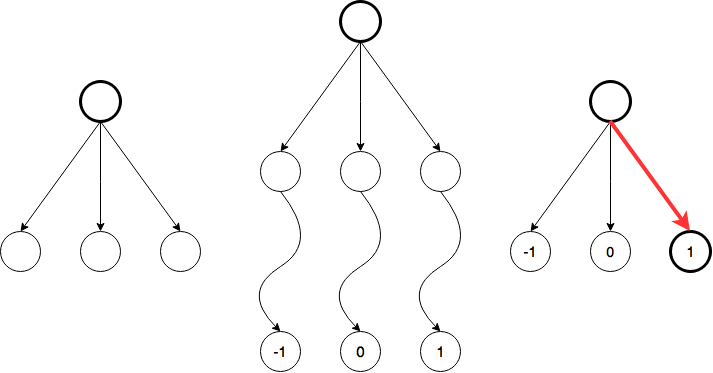
\includegraphics[width=\textwidth]{images/simpleMCTS.png}
\caption{\emph{Example of flat MCS. The right-most action is rated as the best and thus the player chooses to play it.}}
\label{fig:simplemcts}
\end{figure}

The algorithm described in \ref{alg:simmcts} is highly dependant on the random rollouts and thus it is highly likely that the action obtained is not the optimal action. MCS techniques, in general, thus take advantage of repeated simulations in order to obtain more valid approximations to the values of the various actions. 

\subsection{Nested Monte Carlo Search}

Nested Monte Carlo Search (NMCS) is a variant of MCS that uses recursive layers of random simulations in order to determine an optimal move\citebay{cazenave2009nested}. This algorithm (see Algorithm \ref{alg:ncms}) is typically used for 1-player games and thus instead of searching for the best action at a given state, it searches for the whole policy $\pi_{nmcs} = \{s_0, \dots, s_t \}$ \footnote{Here, some liberty is taken in deviating from the definition of the policy $\pi$ as a function. Since NCMS deals with single-player games, it is sufficient to describe $\pi$ as a set of states} where $s_0$ is the initial state and $s_t$ is a possible terminal state. The level $n$ of NMCS defines the depth of recursion that is used in the search. For example a level-0 NMCS algorithm obtains the policy just by performing random rollouts from the initial state until it reaches a terminal state, lines 6 - 10 in the algorithm. NCMS defines utility in terms of policies $R(\pi_{ncms}) \defeq R(s_t)$, i.e, the utility of a policy is the utility of its terminal state. Therefore, NCMS effectively searches to directly find the most optimal terminal state. At higher levels, a level $n$ NCMS algorithm searches for the optimal policy by, for each possible successor state, determining the optimal policy through a level $n-1$ NCMS, lines 14 - 19. The state corresponding to the best optimal policy is chosen as the next state, and the algorithm continues. This idea is illustrated in Figure \ref{fig:nmcs}.
\\
Nested Monte Carlo Search has proven to be an effective algorithm within the domain of single player games such as Morpion, Same Game and Crossword puzzle generation\citebay{cazenave2009nested}. It is because of this success that it is believed that NMCS would be suitable for the problem of first species counterpoint generation.  
 
\begin{figure}[h!]
\centering

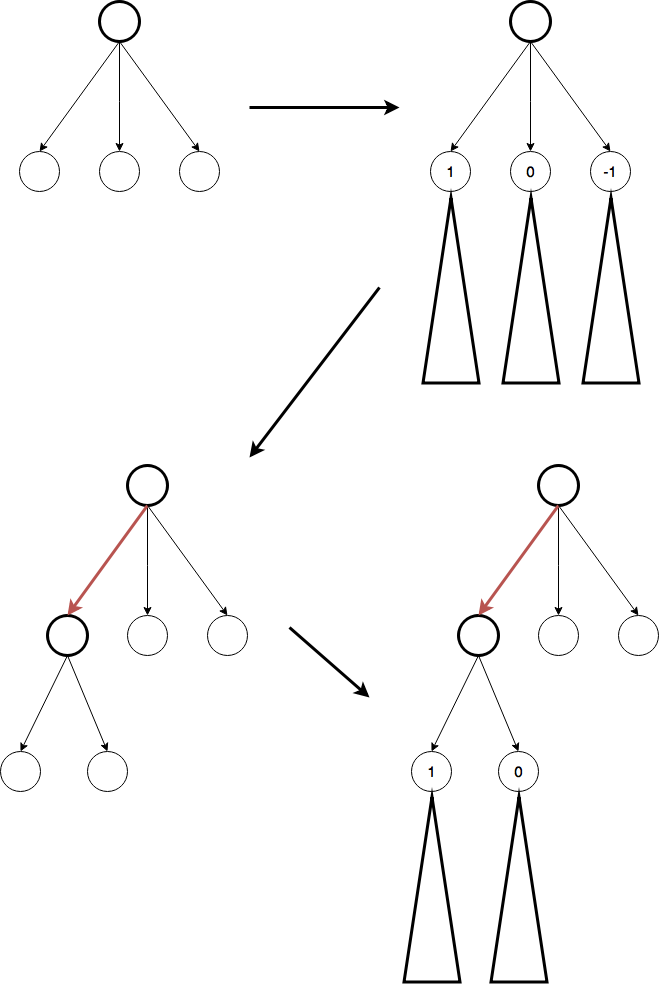
\includegraphics[scale=0.25]{images/NMCS.png}

\caption{\emph{Illustration of the n-level NMCS algorithm. \\The triangles represent an n-1 level NMCS search.}}
\label{fig:nmcs}
\end{figure}

\begin{algorithm}
\caption{Level-n NMCS}
\label{alg:ncms}
\begin{algorithmic}[1]
\Procedure{NCMS}{$n, s$}
\State $ply \gets 0$
\State $\pi \gets \emptyset$
\If {n = 0}
	\State $\pi \gets \{s \}$
	\While {$s \notin S_T$}
		\State $s \gets f(s_{cur}, \textsc{getRandom}(\alpha(s)))$
		\State $\pi.\textsc{add}(s)$
		\State $ply \gets ply + 1$
	\EndWhile
	\State \textbf{return} ($\pi, R(\pi)$)
\Else
	\State $max \gets -\infty$
	\While {$s \notin S_T$}
		\For {$a \in \alpha(s)$}
			\State ($\pi_{temp}, score) \gets NCMS(n - 1,  f(s, a))$
			\If {$score> max$}
				\State $max \gets R(\pi_{temp})$
				\State $\pi.\textsc{add}(s, ply)$
				\State $\pi.\textsc{add}(\pi_{temp}, ply + 1)$
			\EndIf
		\EndFor
		\State $s \gets \pi.\textsc{get}(ply)$
	\EndWhile
	\State \textbf{return} ($\pi, R(\pi)$)
\EndIf
\EndProcedure
\end{algorithmic}
\end{algorithm}

\subsection{Nested Rollout Policy Adaptation} 
Nested Rollout Policy Adaptation (NRPA) is a method based on NMCS created by Rosin \citebay{rosin2011nested}. The algorithm is similar in the sense that it performs nested searches and at level - 0 performs a full playout. The main difference is that, apart from directly traversing the search tree based on the results of previous nested calls, NRPA adapts the rollout policy based on the scores obtained from the nested calls. The idea is that, as search progresses, the policy is updated such that good or promising moves are given increasing probabilities. The algorithm is described in \ref{alg:NRPA}. 

\begin{algorithm}
\caption{Level-n NRPA}
\label{alg:NRPA}
\begin{algorithmic}[1] 
\Procedure{NRPA}{$n, p$}
\If {n = 0} 
	\State $s \gets \text{root()}, ply \gets 0, \pi \gets \emptyset$
	\\
	\While {$s \notin S_T$} 
		 \State $s \gets f(s, \textsc{getRandom}(\alpha (s), p)$
		 \State $\pi.\textsc{add}(s)$
		 \State $ply \gets ply + 1$
	\EndWhile
	\State \textbf{return} ($\pi, R(\pi)$)
\Else
	\State $max \gets -\infty$
	\For {$N$ iterations}
		\State $(\pi_{temp}, score) \gets NRPA(n - 1, p)$
		\\
		\If {$score \geq max$}
			\State $max \gets score$
			\State $\pi \gets \pi_{temp}$
		\EndIf
		\\ 
		\State $p \gets \textsc{adapt}(p, \pi)$
	\EndFor
	\State  \textbf{return} ($\pi, R(\pi)$)
\EndIf
\\
\EndProcedure
\Procedure{adapt}{$p, \pi$}
\State $s \gets  \text{root()}, ply \gets 0, p' \gets p$
\\
\While {$ply < \pi.\textsc{length}()$} 
	\State $s' \gets \pi.\textsc{get}(ply)$
	\State $p'[\textsc{code}(s, s')] \gets p'[\textsc{code}(s, s')]  + \beta$
	\\
	\State $z \gets \sum_{a \in \alpha(s)} \text{exp}(p[code(s, f(s, a))])$
	\\
	\For {$a \in \alpha(s)$}
		\State $p'[code(s, f(s, a))] \gets p'[code(s, f(s, a))] - \frac{\beta}{z}\text{exp}(p[code(s, f(s, a))])$
	\EndFor
	\\
	\State $s \gets s'$
\EndWhile
\State  \textbf{return} $p'$
\EndProcedure
\end{algorithmic}
\end{algorithm}

The algorithm is called with two parameters, $n$ and $p$, the search level and the initial \emph{policy vector}. The policy vector represents the likelihood of an action being selected at a specific state. Therefore, the policy vector must contain a value for each action at each state. These state action pairs are encoded using the function $\textsc{code}(s, s')$, where $s$ represents the current state and $s'$ is the resultant state after applying a specific action.  At level 0, NRPA performs a random playout where each action is chosen proportional to the values in the policy vector, lines 5 - 9. At higher levels, the algorithm searches for $N$ results from $n - 1$ level searches, choosing the best sequence based on its evaluation, lines 12 - 17. The current best sequence is then used to update the values in the policy vector using the $\textsc{adapt}(p, \pi)$ procedure. For all states in the sequence, their weight in the policy vector is increased by a set amount $\beta$. 
\end{document}
\documentclass[master.tex]{subfiles}
\begin{document}
\section{Markov Chains}
Markov Chains (MC) are used to model specific random processes in which transitions between various states occur. The most important property that these processes must possess, is that the transition between one state to another must be \emph{memoryless}. This means that the probability of going from one state to another is independent of the previous states.   This chapter introduces the theory behind MCs and also describes their use within domain of algorithmic music composition. 
\\
\\
Let $S$ be a set of states and assume that there is some process by which random states are selected at discrete time intervals. The sequence of random variables $X_1, X_2, \dots$ represent the random state that is chosen at time interval $1, 2, \dots,$ respectively. A realization of all these random variables $s = (s_1, s_2, \dots)$ is called a \emph{history} which thus represents the states chosen at each time index.  The sequence of random variables is called a \emph{Markov Chain} if they satisfy the \emph{Markov Property}: 

\begin{equation}
\text{Pr}(X_{n+1} = s | X_1 = s_1, X_2 = s_2,\dots, X_n = s_n) = \text{Pr}(X_{n+1} = s | X_n = s_n)
\end{equation}

This property states that the probability of going from one state $s_n$ at time $n$ to another $s_{n+1}$ at time $n + 1$ is dependent on only the previous state $s_n$ and not the history $s = (s_1, s_2, \dots, s_n)$. Further, if the transitional probability from a state $y \in S$ to $x \in S$ is independent of $n$, then the MC is said to be \emph{stationary}.  These stationary Markov Chains can be described using a single matrix $P$ whose entries correspond to transitional probabilities, i.e, $P_{ij} = \text{Pr}(X_2 = j | X_1 = i)$. 
\\
\\
Markov Chains have been used to model the process of music composition by capturing information about transitions between note events in order to generate random pieces with similar structures. The states of the model can be defined using the pitch class values, i.e, $S = (\text{C},\text{C\#}, \text{D}, \dots, \text{B})$. The transitional probabilities of a piece of music would then be determined by calculating the frequencies between various pitch transitions. A new piece is then composed by performing a \emph{random walk} using the probabilities from the transition matrix.

As an example, the melody \emph{Mary had a Little Lamb} is represented by the note sequence $M = \{ E, D, C, D, E, E, E, D, D, D, E, E, E, E, D, C, D, E, E, E, E, D, D, E, D, C\}$. This melody only has 3 distinct pitches so it is sufficient to describe the state space with just $S = (C, D, E)$. An MC built with this melody would then be represented by the following transition matrix. 

\begin{equation}
P = \bordermatrix{~ & C & D & E \cr
				C & 0 & 1 & 0 \cr
				D & \frac{3}{11} & \frac{4}{11} & \frac{4}{11} \cr
				E & 0 & \frac{5}{13} & \frac{8}{13} \cr}
\end{equation}
A caveat to this approach is the fact that most, if not all, music does not possess the Markov Property. The structure of note transitions is highly dependant on the larger scale structure of music as notes play different roles depending on whether they are part of a chord progression, a cadence or the climactic note of phrase. One way to address this issue is to increase the \emph{order} of the MC. The term order refers loosely to the amount of memory an MC has. In an $m$th order MC, the probability distribution for the next state depends on the previous $m$ states. If $m = 1$ we have the MC defined above. Higher order MCs can be described in a similar fashion to first order MCs by increasing the state-space.

 In the previous example, in order to use a second order MC, one would use the state space $S' = ( CC, CD, CE, DC, DD, DE, EC, ED, EE)$. As such, given an original state space of size $|S|$, an $n$th order MC would have a refined state space of size $|S|^{n}$. With higher order MCs, sampled musical pieces will tend to exhibit larger scale structures such as concrete phrases or themes. 
\\
\\
Another issue with modeling music composition with MCs is one that has to do with the state-representation. Using the states as defined above would only be sufficient to model \emph{monophonic} music, music with just one voice. In order to model polyphonic music or harmonies, one needs a different representation. One possible approach would be to use sets of notes as the different states, i.e, one state $s$ could be given by $s = \{F, A, C\}$ to represent that a F major triad was played. If the state space S in such an approach would be limited to a maximum of three pitches per state and only using pitch classes, then $|S| = 12^3 + 12^2 + 12 = 1884$ different states. Creating a transition matrix from a piece of music using such a large state space would result in a very sparse matrix. Sampled music from such a model would thus be very similar if not identical to the original piece. Therefore, in determining a suitable representation, it is necessary to extract features that sufficiently describe the music from a melodic and harmonic point of view. This problem remains an open question, although some attempts have been made to address the issue. In the work of Conklin \citebay{missing} a \emph{vertical viewpoint method} is described. For the purposes of the domain of first species counter point this method would entail representing two pairs of simultaneous notes using three values: two values for the melodic interval between the previous notes and a value for the harmonic interval between the two notes. 
\begin{equation}
\textsc{iv}(a, b) = |b - a|
\end{equation}

In the formula above, a and b represent the (MIDI) pitch values of the notes and thus the interval just represents the amount of semitones between two notes. Using such an approach one could model, for example, which types of intervals typically follow a perfect fifth. Obviously, relying solely on this representation would result in a loss of information about the absolute pitches used in the piece. 
\\
\\
Markov Chains are used in this thesis in order to influence the play-out policy of the Monte Carlo search. Since composing music is such a complex problem, guiding the search towards transitions that have been sampled from existing works is expected to increase the efficiency of the search algorithm. 
\end{document}
\documentclass[master.tex]{subfiles}
\begin{document}
\section{Genetic Algorithms}
Genetic Algorithms (GA) are a class a meta-heuristic search algorithms used for many different types of optimization problems. The main idea behind these algorithms is that they employ a search strategy similar to that of biological evolution and natural selection. This chapter firstly introduces the theory behind GAs and consequently describes how they have been used within the domain of counterpoint generation. 

Being an algorithm inspired by biological phenomena, the theory of GAs has adopted terms from the field of genetics. When defining a GA one first needs to specify what the \emph{genotype} and \emph{phenotype} are. Within biology the genotype refers to the genetic makeup which effectively \emph{encodes} a physical trait, or phenotype. In the case of GA, the distinction is analogous. The genotype is an effective encoding of what the algorithm is optimizing. For the problem of counterpoint generation, one could view the genotype as a sequence of pitches, which represents the phenotype, a phrase of music. Therefore, given a genotype representation, the space of possible genotypes is the search space. An objective or fitness function is a function that takes a genotype and outputs a genotype's fitness, i.e, a measure of how good it is. The idea is thus to find a genotype that maximises the objective function. Genetic Algorithms attempt to find these by using the following procedure. 

\begin{itemize}
\item \textbf{Initialization} \\  
\quad A set of $N$ random genotypes are generated, representing the current \emph{population}. This population represents the first \emph{generation} of candidates.  
\item \textbf{Evaluation} \\ The current population is evaluated according to the objective function. 
\item \textbf{Selection}\\ A selection procedure is employed in order to select $k$ individuals from the current population. Typically the selection procedure randomly selects an individual proportional to their fitness value. Another possible method is to just select the $k$ best individuals. 
\item \textbf{Cross-over} \\ $N$ new individuals are created by recombining the genotypes of two random individuals selected from the $k$ best. The type of recombination is highly domain dependant, although the idea is to be able to retain and combine the information of the two individuals so that the new genotype has an equal or better fitness. 
\item \textbf{Mutation} \\ For each of the $N$ new individuals, their genotype is mutated by some probability $\alpha$. This mutation usually entails changing a small part of the genotype. For example, if a binary representation is used, mutation would change the value of a bit with probability $\alpha$. Mutations are used in order to try to prevent the algorithm from prematurely converging on local maxima\citebay{geneticcitation}. Higher values of $\alpha$ will result in more exploration of the search space although it will take longer for the problem to converge at a optimal solution \citebay{citation}.  
\item \textbf{Repeat} \\ The algorithm returns to the evaluation phase and the process continues until some stopping criteria is reached. Again, this criteria is highly domain dependant. As an example, one could stop searching when there is no change between the maximum fitness value of two generations. 
\end{itemize} 
Genetic Algorithms have seen a number of sucesses in various applications. In particular, they have become a popular go to method for various problems algorithmic composition \citebay{}.   
\\
\textbf{TODO: add more information about literature of GA successes within the domain of music composition}. 
\\
In order to determine how well the Monte Carlo based approach fares within the domain, it was tested against a Genetic Algorithms within the domain of first species counterpoint generation. To this end a Genetic Algorithm similar to ones found in the literature was defined. The specifics of the algorithm are found in a subsequent chapter. 
\end{document}
\chapter{Related work}

\chapter{Experiments}

\chapter{Results}

\chapter{Conclusions}

\bibliography{bib} \emptypage

\appendix

\appchapter{Algorithms}

\appchapter{Detailed results}


\chapterx{Samenvatting} \emptypage

% this can be a translation of the abstract

\end{document}
